%!TEX TS-program = xelatex
%!TEX encoding = UTF-8 Unicode

\documentclass[8pt]{article}
\usepackage[a4paper]{geometry}
\usepackage[english]{babel}
\usepackage{amssymb,amsthm,amsmath}
%\usepackage{xltxtra}
%\usepackage{stmaryrd}
\usepackage{tikz}
\usepackage{graphicx}
\usepackage{listings}
\usepackage{color}

\graphicspath{ {./images/} }

\definecolor{universityred}{RGB}{147,25,50}
\definecolor{complementaryb}{RGB}{25,147,122}
\definecolor{complementaryo}{RGB}{246,152,84}
\definecolor{complementaryg}{RGB}{110,147,25}

\lstset{
	extendedchars=true,
	showstringspaces=false,
	escapeinside=``,
	keywordstyle=\color{blue},
	commentstyle=\color[rgb]{0.133,0.545,0.133},
	columns=flexible,
	language=python,
	tabsize=2,
	basicstyle=\normalsize\selectfont\ttfamily,
	numbers=left,
	frame=lines,
	breaklines=true
}
\geometry{
	left=15mm,
	right=7mm,
	top=7mm,
	bottom=15mm
}
\usepackage{multicol}
\setlength{\columnsep}{1cm}


\begin{document}
\begin{titlepage}
    \begin{center}
        \vspace*{1cm}

        \Huge
        \textbf{SWERC NoteBook}

        \vspace*{0.5cm}
        \LARGE
        \'Equipe SaintGermainDesPrés

        \normalsize
        \vspace*{1.5cm}
        \textbf{Mathilde BONIN, Eyal COHEN, Hugo DEMARET}

        \vspace*{1cm}
        \textbf{Avril 2022}

        \vspace*{2.5cm}

        \LARGE
        \textbf{Ensemble d'algorithmes et techniques de programmation}\\
        \textit{Et quelques notions de Mathématiques}
        \vspace*{3.cm}

        
        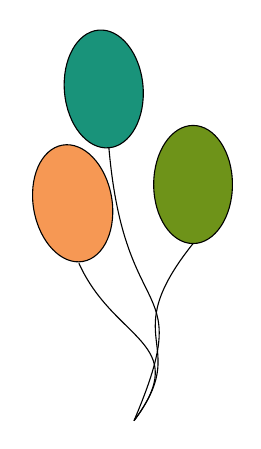
\begin{tikzpicture}
            \filldraw[fill=complementaryg, draw=black](0,2) ellipse (.5cm and .75cm);
            \draw (-0.75,-1) .. controls (0,0) and (-1.,0) .. (0,1.25);
            \draw (-0.75,-1) .. controls (0,0) and (-1.,0) .. (-1.45,1);
            \draw (-0.75,-1) .. controls (0.1,1) and (-1.,0) .. (-1.1,3);
            \draw[rotate around={10:(0,0)},fill=complementaryo, draw=black] (-1.2,2) ellipse (.5cm and .75cm);
            \draw[rotate around={5:(0,0)},fill=complementaryb, draw=black] (-0.85,3.3) ellipse (.5cm and .75cm);
        \end{tikzpicture}

        
\includegraphics[scale=0.05]{../image/cover_image.png}
        \Large
        \vspace{2cm}

        \textbf{Université Paris Cité}\\
        UFR de Mathématiques-Informatique

        2021-2022

    \end{center}
\end{titlepage}
    \section{Configuration}
        \subsection{C/C++}
        
    \section{Chaînes de caractères}
    \section{Séquences}
        \subsection{Anagramme}
        {\scriptsize\lstinputlisting{../code/string/anagramme.py}}
        \subsection{Distance de Levenshtein}
        {\scriptsize\lstinputlisting{../code/string/levenshtein.py}}
        \subsection{Plus grand facteur commun}
        {\scriptsize\lstinputlisting{../code/string/longest_common_subsequence.py}}
        \subsection{Rabin-Karp | Recherche d'un pattern}
        {\scriptsize\lstinputlisting{../code/string/rabin_karp.py}}
    \section{Parcours de graphes}
        \subsection{DFS - Depth First Search}
        {\scriptsize\lstinputlisting{../code/graphes/dfs.py}}
        \subsection{BFS - Breadth First Search}
        {\scriptsize\lstinputlisting{../code/graphes/bfs.py}}
        \subsection{Topological Sort}
        {\scriptsize\lstinputlisting{../code/graphes/topological_sort.py}}
        \subsection{Composantes connexes}
        \subsection{Composantes bi-connexe}
        {\scriptsize\lstinputlisting{../code/graphes/bi_connected_components.py}}
        \subsection{Composantes fortement connexe}
            \subsubsection{Kosaraju}
            {\scriptsize\lstinputlisting{../code/graphes/kosaraju_dfs.py}}
        \subsection{2-SAT}
        {\scriptsize\lstinputlisting{../code/graphes/two_sat.py}}
        \subsection{Postier Chinois}
        \subsection{Chemin eulérien}
            \subsubsection{Dirigé}
            {\scriptsize\lstinputlisting{../code/graphes/eulerian_tour_directed.py}}
            \subsubsection{Non Dirigé}
            {\scriptsize\lstinputlisting{../code/graphes/eulerian_tour_undirected.py}}
        \subsection{Chemin le plus court}
            \subsubsection{Poids positif ou nul - Dijkstra}
            {\scriptsize\lstinputlisting{../code/graphes/dijkstra.py}}
            \subsubsection{Poids arbitraire - Bellman-Ford}
            {\scriptsize\lstinputlisting{../code/graphes/bellman_ford.py}}
            \subsubsection{Floyd-Warshall}
            {\scriptsize\lstinputlisting{../code/graphes/floyd_warshall.py}}
    \section{Points et polygones}
        \subsection{Points}
            \subsubsection{Points}
            {\scriptsize\lstinputlisting{../code/points/point.py}}
            \subsubsection{Cross-product}
            {\scriptsize\lstinputlisting{../code/points/crossproduct.py}}
            \subsubsection{Direction}
            {\scriptsize\lstinputlisting{../code/points/direction.py}}
        \subsection{Enveloppe convexe}
            Complexité : $\mathcal{O}(n \log(n))$
            {\scriptsize\lstinputlisting{../code/points/jarvismarch.py}}
        \subsection{Aire d'un polygone}
        \textit{Uniquement pour les polygones simples. Réduire à des composantes simples sinon.}
        Voir partie Mathématiques.
        {\scriptsize\lstinputlisting{../code/points/polygonearea.py}}
        \subsection{Polygone simple}
        {\scriptsize\lstinputlisting{../code/points/simple_polygon.py}}
        \subsection{Paire de points les plus proches}
    \section{Ensembles}
        \subsection{Rendu de monnaie}
        Problème NP-Complet.
        {\scriptsize\lstinputlisting{../code/ensembles/coin.py}}
        \subsection{Sac à dos}
        Problème NP-Complet.
        {\scriptsize\lstinputlisting{../code/ensembles/knapsack.py}}
        \subsection{k-somme}
        \subsection{Points les plus proches}
        {\scriptsize\lstinputlisting{../code/ensembles/closest_points.py}}
        \subsection{Valeurs les plus proches}
        {\scriptsize\lstinputlisting{../code/ensembles/closest_values.py}}
    \section{Calculs}
        \subsection{PGCD}
        {\scriptsize\lstinputlisting{../code/calculs/pgcd.py}}
        \subsection{Coefficients de Bézout}
        {\scriptsize\lstinputlisting{../code/calculs/bezout.py}}
        \subsection{Coefficients binomiaux}
        {\scriptsize\lstinputlisting{../code/calculs/binom.py}}
        \subsection{Inverse}
        {\scriptsize\lstinputlisting{../code/calculs/inverse.py}}
    \section{Mathématiques}
        \subsection{Géométrie}
            \subsubsection{3D}
            \begin{itemize}
                \item Sphère : Volume : $\frac{4}{3}\pi r^{3}$ | Surface : $4\pi r^{2}$
                \item Cylindre droit : Volume $\pi r^{2} h$ | Surface : $2\pi r( r + h)$
                \item Cone circulaire droit : Volume $\frac{1}{3} \pi r^{2} h$ | Surface : $\pi r( r + s)$
                \item Prisme triangulaire : Volume $A  l$ ou $\frac{1}{2}bhl$ | Surface : $bh + 2ls + lb$
                \item Prisme : Volume $Ah$ | Surface : $2A + (h \times p)$
                \item Pyramide : Volume : $\frac{1}{3}Ah$
                \item Tétrahèdre : Volume : $\frac{b^{3}}{6  \sqrt[2]{2}}$ | Surface : $\sqrt[2]{3}b^{2}$
                \item Pyramide carré : Volume : $\frac{1}{3}s^{2}\times h$ | Surface : $s^{2} + 2sh$
                \item Cuboide : Volume : $l\times w \times h$ | Surface : $2lh + 2lw +2wh$ (Cube : $6s^{2}$)
            \end{itemize}
            \subsubsection{2D}
            \begin{itemize}
                \item Polygone simple : Aire : $A = \frac{1}{2} \sum_{i=0}^{n-1}\left(x_{i}x_{i+1} - x_{i+1}y_{i}\right)$
                \item Cercle : Aire : $\pi r^{2}$ | Périmètre : $2\times \pi \times r$
                \item Losange : Aire : $\frac{D\times d}{2}$
                \item Trapèze : Aire : $\frac{(B+b)\times h}{2}$
                \item Parralélogramme : Aire : $B\times h$
            \end{itemize}
            \subsubsection{Points entiers dans un polygone}
                Sur le contour : \\
                Dans le polygone : \\
                Théorème de Pick :
                $P = n_{i} + \frac{n_{b}}{2}-1$
            \subsubsection{Théorème de la galerie d'art}
            Pour garder un polygone simple à $n$ sommets, $\lfloor \frac{n}{3} \rfloor$ gardiens suffisent.
        \subsection{Approximations}
            \subsubsection{Méthode de Newton}
            $x_{k+1} = x_{k} - \frac{f(x_{k})}{f'(x_{k})}$ | $f(x) \approx f(x_{0}) + f'(x_{0})(x-x_{0})$
            \subsubsection{Méthode de la sécante}
            Cette méthode est à appliquer quand le calcul de la dérivée est couteux
            $\frac{f(x_{k} )- f(x_{k-1})}{x_{k} - x_{k-1}}$
            \subsubsection{Plus forte pente | Méthode du gradient}
            Cette méthode peut être assez couteuse (ZigZag) \\
            \textbf{Algorithme du gradient} | On se donne un point initial $x_0 \in \mathbb{E}$ et un seuil de tolérance
            $\epsilon \geq 0$. L'algorithme du gradient donne une suite d'itérés $x_1 , x_2 ... \in \mathbb{E}$, jusqu'à ce qu'un test d'arrêt
            soit satisfait. Il passe de $x_k$ à $x_{k+1}$ par les étapes suivantes :
            \begin{itemize}
                \item 1. \textit{Simulation} : Calcul de $\nabla f(x_k)$
                \item 2. \textit{Test d'arrêt} : Si $\lVert \nabla f(x_k) \rVert \leq \epsilon$, arrêt 
                \item 3. \textit{Calcul du pas} : $\alpha_k > 0$ par un règle de recherche linéaire sur $f$ en $x_k$
                le long de la direction $-\nabla f(x_k)$
                \item 4. \textit{Nouvel itéré} : $x_{k+1} = x_k - \alpha_k \nabla f(x_k)$ 
            \end{itemize}
        \subsection{Probabilités et Statistiques}
            \subsubsection{Lois de probabilités}
            Discrètes :
                \begin{itemize}
                    %$\mathbb{P}(X=k) = , \quad \mathbb{E}[X] = , \quad \mathbb{V}[X] = $
                    \item Poisson : $\mathbb{P} (X=k) = e^{-\lambda}\frac{\lambda^k}{k!}, \quad \mathbb{E}[X]=\lambda, \quad \mathbb{V}[X]=\lambda$
                    \item Binomiale : $\mathbb{P}(X=k) = \binom{n}{k} p^k (1-p)^{n-k}, \quad \mathbb{E}[X] = np, \quad \mathbb{V}[X] = np(1-p)$
                    \item Géométrique : $\mathbb{P}(X=k) = (1-p)^{k-1}p, \quad \mathbb{E}[X] = \frac{1}{p}, \quad \mathbb{V}[X] = \frac{1-p}{p^{2}}$
                    \item Uniforme : $\mathbb{P}(X=k) = \frac{1}{n}, \quad \mathbb{E}[X] = \frac{1}{n}  \sum^{n}_{k=1} x_k$
                \end{itemize}
            \subsubsection{Techniques statistiques}
            Théorème de la limite centrale : \\
            Soit $X_1,X_2,...$ une suite de variable aléatoires réelles définies sur le même espace de probabilités, i.i.d et suivant la même loi $\mathcal{L}$.
            De plus, l'espérance $\mu$ et l'écart-type $\sigma$ de $\mathcal{L}$ existent et soient finis avec $\sigma \neq 0$.\\
            Soit la somme $S_n = X_1 + X_2 + ... + X_n$\\
            Alors l'espérance de $S_n$ est $n\mu$ et l'écart-type est $\sigma \sqrt{n}$\\
            Quand $n$ est assez grand, la Loi Normale $\mathcal{N}(n\mu,n\sigma^{2})$ est une bonne approximation de $S_n$\\
            On pose $\overline{X_n} = \frac{S_n}{n}$ et $Z_n = \frac{S_n-n\mu}{\sigma \sqrt{n}} = \frac{\overline{X_n}-\mu}{\sigma / \sqrt{n}}$
    \section{Techniques de programmation}
        \subsection{Programmation dynamique}
        Résoudre le problème en le divisant en sous-problèmes, résoudre les sous-problèmes, stocker les résultats
        intermédiaires ("mémoisation")
        \subsection{Diviser pour régner}
        Diviser un problème en sous-problèmes; Résoudre les sous-problèmes; Combiner : calculer la solution grâce aux
        solutions des sous-problèmes.
        \subsection{Floyd's Hare and Tortoise}
        L'objectif de cette méthode est de détecter des cycles. L'idée est de parcourir la liste chaînée
        avec deux pointeurs : un lent (tortoise) et un deux fois plus rapide (hare). Si les deux pointeurs
        s'intersectent, il y a un cycle.
\end{document}